% Author: Izaak Neutelings (December 2020)
% Inspiration: https://tex.stackexchange.com/questions/285578/how-to-draw-parallelepiped-and-cube-with-latex/288101#288101
\documentclass[border=3pt,tikz]{standalone}
\usepackage{amsmath}
\usetikzlibrary{arrows,arrows.meta}
\tikzset{>=latex} % for LaTeX arrow head

\colorlet{myblue}{blue!60!black}
\colorlet{myred}{red!80!black}
\colorlet{vcol}{green!60!black}
\tikzstyle{vvec}=[-{Latex[length=4,width=3]},thick,vcol,line cap=round]
\tikzstyle{myarr}=[-{Latex[length=3,width=2]}]
\tikzstyle{mydoublearr}=[{Latex[length=3,width=2]}-{Latex[length=3,width=2]}]
\tikzset{
  pics/eye/.style={
    code={
      \draw (#1-180:0.5) to[out=#1,in=#1-240,looseness=0.9] (#1-90:0.25)
            (#1-180:0.5) to[out=#1,in=#1-130,looseness=0.9] (#1-270:0.25);
      \clip (#1-180:0.47) to[out=#1,in=#1-240,looseness=0.9] (#1-90:0.24) --
            (#1-270:0.242) to[out=#1-130,in=#1,looseness=0.9] cycle;
      \draw[very thin,top color=white,bottom color=red!60!black!20,shading angle=#1-120]
         (#1-180:0.48) circle(0.45);
      \fill[brown!30!black,rotate=#1-180]
        (0.07,0) ellipse({0.05} and 0.12);
      \fill[black,rotate=#1-180]
        (0.05,0) ellipse({0.03} and 0.06);
  }},
  pics/eye/.default=180
}

\begin{document}

% REST
\def\R{1.5}      % radius
\def\N{5}        % number of wave fronts
\def\lam{\R/\N}  % wavelength
\def\angmin{30}  % min. angle velocity arrow
\def\angmax{330} % min. angle velocity arrow
\def\waves#1{
  \foreach \i in {1,...,\N}{
    \draw[myblue,thick] ({-(\i-0.25)*#1*\lam},0) circle ({\lam*(\i-0.25)});
  }
  \foreach \a in {\angmin,90,150,210,270,\angmax}{
    \draw[myarr,vcol] ({-(\N-0.25)*#1*\lam},0)++(\a:\R-0.50*\lam) --++ (\a:\lam);
  }
  \fill[myred] (0,0) circle (0.06);
}
\begin{tikzpicture}
  \waves{0}
  \node[vcol] at (30:1.22*\R) {$c$};
  \draw[mydoublearr]
    (-0.9*\R,-0.8*\R) node[left=-1,scale=0.7] {$y$}
    |-++ (0.15*\R,-0.15*\R) node[right=-1,scale=0.7] {$x$};
  \begin{scope}[shift={(0,-1.35*\R)}]
    \draw[myblue,thick,samples=100,smooth,variable=\x]
      plot[domain=-\R:0](\x,{0.1*\R*sin(360/(\lam)*\x)}) %--
      plot[domain=0:\R](\x,{-0.1*\R*sin(360/(\lam)*\x)});
    \fill[myred] (0,0) circle (0.05);
    \draw[myarr,vcol] (-\R+0.25*\lam,0.04*\R) --++ (-\lam,0);
    \draw[myarr,vcol] (\R-0.25*\lam,0.04*\R) --++ (\lam,0);
    \draw[mydoublearr]
      (-\R-2.3*\lam,0.06*\R) node[left=-1,scale=0.7] {$z$}
      |-++ (0.15*\R,-0.15*\R) node[right=-1,scale=0.7] {$x$};
  \end{scope}
\end{tikzpicture}

% MOVING - DOPPLER SHIFT
\begin{tikzpicture}
  \def\s{0.61}
  \draw[myblue!20,dashed,very thin,dash pattern=on 1 off 1]
    ({-(\N-0.25)*\s*\lam},0) -- (0,0);
  \fill[myred!20] ({-(\N-0.25)*\s*\lam},0) circle (0.06);
  \waves{\s}
  \node[vcol] at (30:{1.15*\R-\s*\R} and 1.2*\R) {$c$};
  \draw[mydoublearr]
    (-0.9*\R-\s*\R,-0.8*\R) node[left=-1,scale=0.7] {$y$}
    |-++ (0.15*\R,-0.15*\R) node[right=-1,scale=0.7] {$x$};
  %\draw[dashed] (\R-\s*\R,0) --++ (0,-1.3*\R);
  %\draw[dashed] (0,0) --++ (0,-1.3*\R);
  %\draw[dashed] (-\R-\s*\R,0) --++ (0,-1.3*\R);
  \pic at ( 1.25*\R-\s*\R,0) {eye={180}};
  \pic at (-1.15*\R-\s*\R,0) {eye={0}};
  \draw[-{Latex[length=4.8,width=3.8]},white,line width=1.2]
    (0.05,0) -- (0.22*\R+0.02,0);
  \fill[myred] (0,0) circle (0.06);
  \draw[-{Latex[length=4,width=3]},thick,vcol,line cap=round]
    (0.05,0) -- (0.22*\R,0); %node[right=-1] {$v$};
  \begin{scope}[shift={(0,-1.35*\R)}]
    \draw[myblue,thick,samples=100,smooth,variable=\x]
      plot[domain=-(\s+1)*(\R):0](\x,{0.1*\R*sin(360/(\s+1)/(\lam)*\x)}) %--
      plot[domain=0:(1-\s)*(\R)](\x,{-0.1*\R*sin(360/(1-\s)/(\lam)*\x)});
    \fill[myred] (0,0) circle (0.05);
    \draw[myarr,vcol] ({-(\s+1)*(\R-0.25*\lam)},0.04*\R) --++ (-\lam,0);
    \draw[myarr,vcol] ({(1-\s)*(\R-0.25*\lam)},0.04*\R) --++ (\lam,0);
    \draw[mydoublearr]
      (-\R-\s*\R-2.3*\lam,0.06*\R) node[left=-1,scale=0.7] {$z$}
      |-++ (0.15*\R,-0.15*\R) node[right=-1,scale=0.7] {$x$};
  \end{scope}
  %\draw[<->] (0,-1.5*\R) --++ (\R-\s*\R,0)
  %  node[midway,right=2,below=1,scale=0.6] {$\sim c-v$}; %{$\sim\dfrac{c}{c+v}$};
  %\draw[<->] (0,-1.5*\R) --++ (-\R-\s*\R,0)
  %  node[midway,below=1,scale=0.6] {$\sim c+v$}; %{$\sim\dfrac{c}{c-v}$};
\end{tikzpicture}

% DOPPLER SHIFT - distances
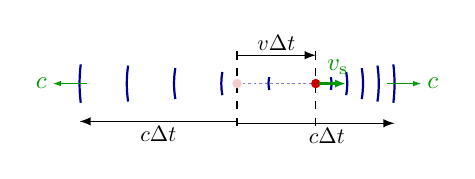
\begin{tikzpicture}
  \def\R{2.0}     % total radius
  \def\N{5}       % number of wave fronts
  \def\lam{\R/\N} % wavelength
  \def\s{0.5}     % shift
  \def\ang{13}    % opening angle
  \draw[dashed]
    (-\s*\R,-0.27*\R) --++ (0,0.5*\R)
    (0,-0.27*\R) --++ (0,0.5*\R);
  \draw[myblue!50,dashed,very thin,dash pattern=on 1 off 1]
    ({-\s*\R},0) -- (0,0);
  \fill[myred!20] ({-\s*\R},0) circle (0.06);
  \foreach \i [evaluate={\r=\i*\lam;\a=\ang-1.2*\i;}] in {1,...,\N}{
    \draw[myblue,thick] ({-\i*\s*\lam},0)++(180-\a:\r) arc(180-\a:180+\a:\r);
    \draw[myblue,thick] ({-\i*\s*\lam},0)++(    \a:\r) arc(    \a:-\a:\r);
  }
  \draw[white,line width=1.2] %-{Latex[length=4.8,width=3.8]}
    (0.05,0) -- (0.96*\lam-0.02,0);
  \fill[myred] (0,0) circle (0.06);
  \draw[-{Latex[length=4,width=3]},thick,vcol,line cap=round]
    (0.05,0) -- (0.96*\lam,0) node[left=3,above=0,scale=0.9] {$v_\mathrm{s}$};
  \draw[->] (-\s*\R,0.18*\R) --++ (\s*\R,0)
    node[midway,above=-1,scale=0.8] {$v\Delta t$};
  \draw[->] (-\s*\R,-0.252*\R) --++ (\R,0)
    node[midway,right=4,below=-1,scale=0.8] {$c\Delta t$};
  \draw[->] (-\s*\R,-0.240*\R) --++ (-\R,0)
    node[midway,below=-1,scale=0.8] {$c\Delta t$};
  \draw[myarr,vcol] (0:\R-\s*\R-0.25*\lam) --++ (0:1.1*\lam) node[right=-1,scale=0.9] {$c$};
  \draw[myarr,vcol] (180:\R+\s*\R-0.25*\lam) --++ (180:1.1*\lam) node[left=-1,scale=0.9] {$c$};
\end{tikzpicture}

% SONIC BOOM
\begin{tikzpicture}
  %\draw[red!60!black!90,dash pattern=on 2 off 2,thin]
  %  (0.05,0.2*\R) --++ (0,-0.4*\R);
  \waves{0.97}
\end{tikzpicture}

% SUPERSONIC
\begin{tikzpicture}
  \def\angmin{90}  % min. angle velocity arrow
  \def\angmax{270} % min. angle velocity arrow
  \def\f{1.4}
  \def\ang{asin(1/\f)}
  \waves{\f}
  \draw[red!60!black!90,dash pattern=on 2 off 2,thin]
    (0.015,0)++({180-\ang}:0.045) --++ ({180-\ang}:1.45*\R)
    (0.015,0)++({180+\ang}:0.045) --++ ({180+\ang}:1.45*\R);
  \foreach \i in {2,4,6}{
    \draw[myarr,vcol] ({-(\i-0.25)*\f*\lam},0)++({90-\ang}:{\lam*(\i-0.45)}) --++ ({90-\ang}:\lam);
    \draw[myarr,vcol] ({-(\i-0.25)*\f*\lam},0)++({\ang-90}:{\lam*(\i-0.45)}) --++ ({\ang-90}:\lam);
  }
\end{tikzpicture}

\end{document}